\subsection{Einleitung}
\begin{itemize}
\item Gleichstrommaschinen werden bis ca. 3kV Nennspannung und bis zu einer Leistung von 20 MW hergestellt.
\item Gleichstrommaschinen werden heute häufig in dynamischen Bereichen, mit ständig ändernden Drehzahlen in weiten Bereichen eingesetzt.
\end{itemize}

\subsection{Aufbau und Wirkungsprinzip}
\begin{minipage}{0.5 \linewidth}
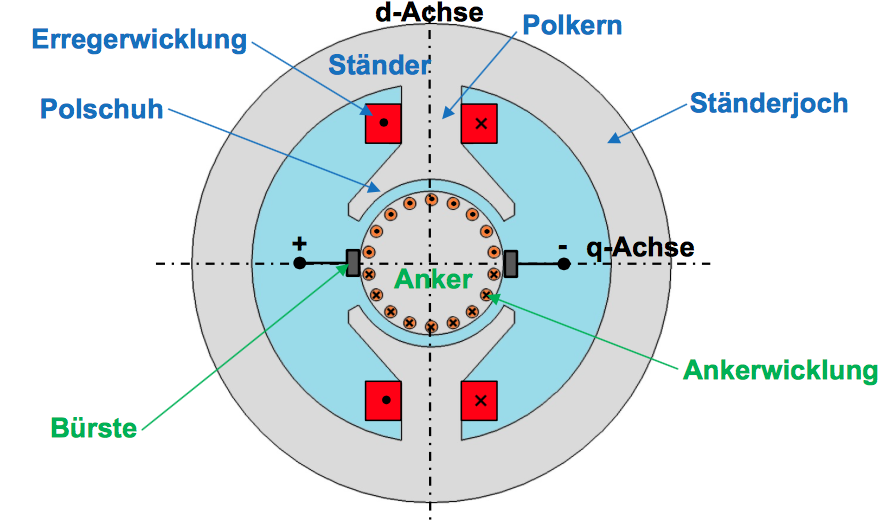
\includegraphics[width = \linewidth]{./Pics/VL45/GSMAufbau}
\end{minipage}
\begin{minipage}{0.5 \linewidth}
\begin{itemize}
\item Die vom Gleichstrom durchflossene Erregerwicklung erzeugt das magnetische Hauptfeld der Maschine.
\item Das Ständerjoch, der Polkern, der Polschuh und der Ankerkern sind aus lamelliertem Eisen gefertigt, weil Eisen magnetische Feldlinien viel besser als Luft ($\mu_{rFE} \approx 10^5$) führt. 
\item Der magnetische Fluss fliesst durch den Kern des Ständers, überspringt den Luftspalt zwischen dem Polschuh und Rotor und geht weiter durch den Kern des Rotors.
\item \textbf{Gleichstromgenerator:} Durch die Umdrehung der Ankerwicklung im magnetischen Hauptfeld wird die Wechselspannung in den Wicklungen induziert. Die Induzierte Spannung der Ankerwicklung wird mit den Bürsten und Schleifringen (Kommutator) gleichgerichtet und nach aussen geführt.
\item \textbf{Gleichstrommotor:} Eine Gleichstromquelle wird über den Kommutator mit den Ankerwicklungen verbunden. Wenn der elektrische Strom durch die Ankerwicklung im magnetischen Hauptfeld fliesst, wird denn die auf die Ankerwicklung wirkende magnetische Kraft (d.h. das Moment des Motors) erzeugt. 
\end{itemize}
\end{minipage}

\subsubsection{Wirkungprinzip GSM-Motor}
Wenn der elektrische Strom durch die Ankerwicklung im magnetischen Hauptfeld fliesst, wird die auf die Ankerwicklung wirkende magnetische Kraft (d.h. das Moment des Motors) erzeugt:

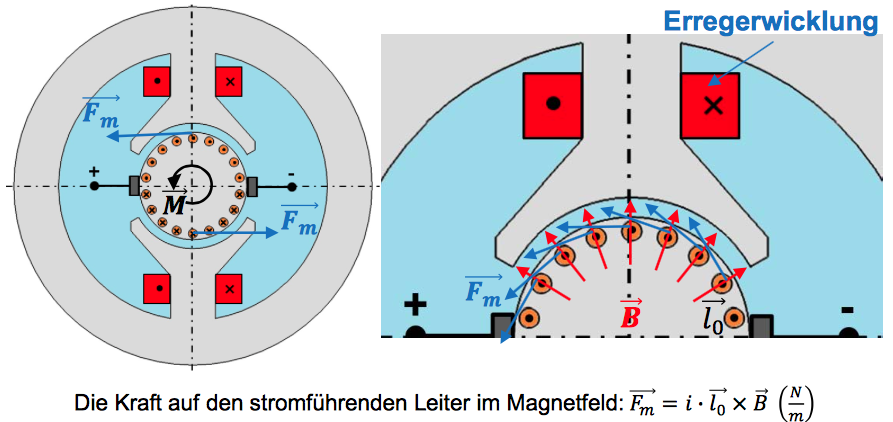
\includegraphics[width = 0.8 \linewidth]{./Pics/VL45/GSMMotor}

\subsection{Grundgleichungen, Kommmutierung, Ersatzschaltbild}
\begin{minipage}{0.3 \linewidth}
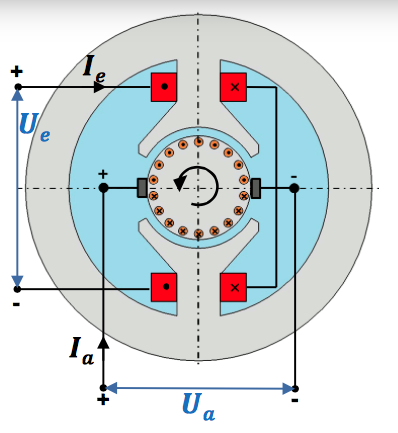
\includegraphics[width = \linewidth]{./Pics/VL45/GSM}
\end{minipage}
\begin{minipage}{0.6\linewidth}
Die Erregerwicklung, die den Erregerwiderstand $R_e$ und die Erregerinduktivität $L_e$ besitzt, wird an die Spannungsquelle $U_e$ angeschlossen. Gemäss dem zweiten Kirchooffschen Gesetz sind die Erregerspannung $U_e$ und der Erregerstrom $I_e$ wie folgt verknüpft: \\

$U_e = R_e \cdot I_e + L_e \cdot \frac{dI_e}{dt}$ \\

Ebenso weisst die Ankerspule im Läuferkreis den Ankerwiderstand $R_a$ und die Ankerinduktivität $L_a$ auf. Im Gegensatz zu der Erregerwicklung dreht sich die Ankerspule im magnetischen Hauptfeld um und dadurch wird in dieser Spule eine zusätzliche Spannung $E$ induziert, die im Ankerkreis eine wichtige Rolle spielt: \\

$U_a = R_a \cdot I_a + L_a \cdot \frac{dI_a}{dt} + E$
\end{minipage}

\begin{minipage}{0.25 \linewidth}
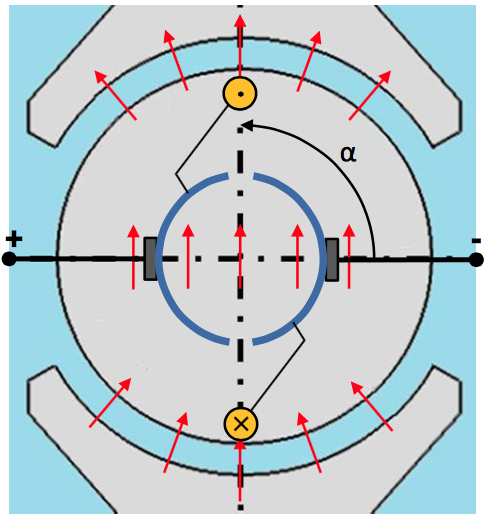
\includegraphics[width = \linewidth]{./Pics/VL45/GSM2}
\end{minipage}
\begin{minipage}{0.7\linewidth}
\begin{itemize}
\item Um die Kommutierung des Ankerstroms zu erklären ist nur eine Anker-Leiterschleife (gelb) dargestellt. Die beiden Enden der Schleife sind mit den zwei seperaten Schleifringen (blau) verbunden. Die Schleifringe zusammen mit den anliegenden Bürsten werden als Kommutator oder Stromwender gennant.
\item Die Stromführung zwischen dem äusseren elektrischen System und den rotierenden Ankerspulen ermöglichen die durch Federdruck gepressten Kohlebürsten.
\end{itemize}
\end{minipage}


\begin{minipage}{0.4 \linewidth}
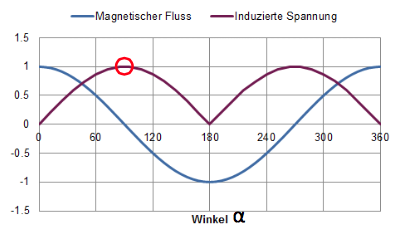
\includegraphics[width = \linewidth]{./Pics/VL45/GSM3}
\end{minipage}
\begin{minipage}{0.6\linewidth}
Die Position der Bürsten ist sehr wichtig für die verlustfreie Kommutierung. Wenn eine Bürste gleichzeitig die beiden Schleifringe berührt ($\alpha = 180^\circ$), muss in diesem Moment die induzierte Spannung der entsprechenden Wicklungsektion gleich Null werden. Sonst werden Lichtbögen zwischen den Lamellen des Kommutators entstanden, was als Läuferfeuer bekannt ist. Das Läuferfeuer ist ein klares Anzeichen der schlechten Kommutierung, die die Lebensdauer der Maschine wesentlich verkürzen könnte.
\end{minipage}

\subsection{Ersatzschaltbild}
\begin{minipage}{0.4 \linewidth}
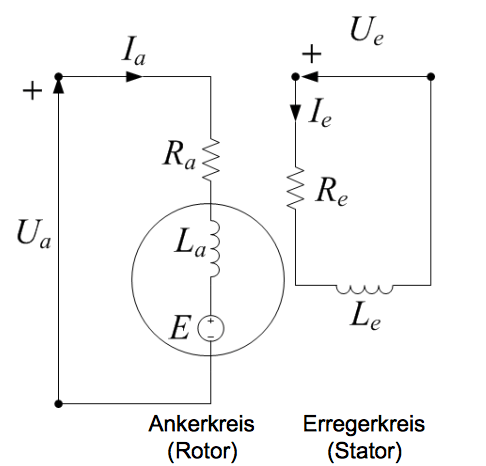
\includegraphics[width = \linewidth]{./Pics/VL45/GSMErsatzschaltbild2}
\end{minipage}
\begin{minipage}{0.6\linewidth}
Die Spannungsgleichung des Statorkreises: \\

$U_e = R_e \cdot I_e + L_e \cdot \frac{dI_e}{dt}$ \\

Die Spannungsgleichung des Rotorkreises: \\

$U_a = R_a \cdot I_a + L_a \cdot \frac{dI_a}{dt} + E $\\

Die induzierte Spannung der Ankerwicklung lässt sich so angeben: \\

$E = \omega \cdot \Psi$\\

wobei $\omega = 2 \cdot \pi \cdot n / 60$ die Winkelgeschwindigkeit des Läufers, $n$ die Drehzahl des Läufers, und $\Psi$ der verkettete Erregerfluss ist. 
\end{minipage}

\subsection{Drehmoment}
\begin{minipage}{0.4 \linewidth}
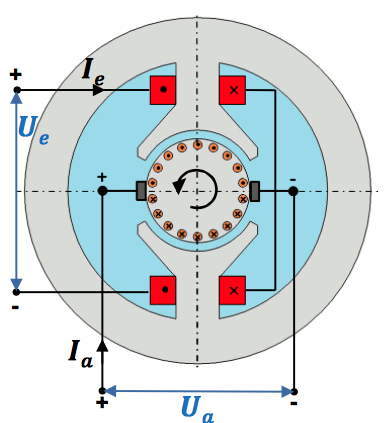
\includegraphics[width = \linewidth]{./Pics/VL45/GSMErsatzschaltbild}
\end{minipage}
\begin{minipage}{0.6 \linewidth}
Die elektrische Leistung der Maschine im stationären Betrieb ($\frac{d}{dt} = 0$) lässt sich wie folgt angeben: \\

$P_{el} = P_e + P_a = U_e \cdot I_e + U_a \cdot I_a$ ($W$) \\

$P_{el} = R_e \cdot I_e^2 + R_a \cdot I_a^2 + \omega \cdot \Psi \cdot I_a$ ($W$) \\

$R_e \cdot I_e^2$  - Ohmsche Erregerverluste \\

$R_a \cdot I_a^2$  - Ohmsche Ankerverluste \\

$\omega \cdot \Psi \cdot I_a$ -  Mechanische Leistung \\

$P_mech = \omega \cdot M$ ($W$), wobei M das Drehmoment ist. \\

$M = \Psi \cdot I_a$ ($Nm$)
\end{minipage}

\subsection{Ankerrückwirkung}
\begin{minipage}{0.4 \linewidth}
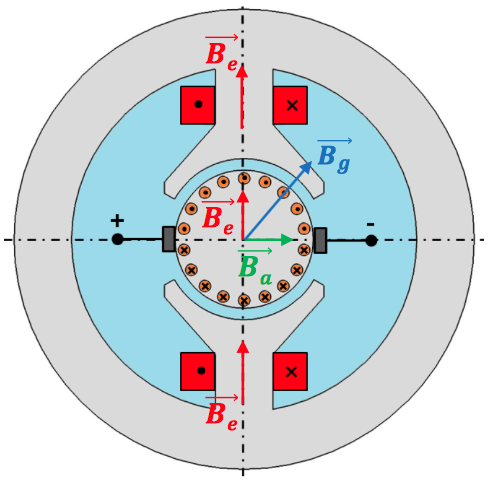
\includegraphics[width = \linewidth]{./Pics/VL45/Ankerruek}
\end{minipage}
\begin{minipage}{0.6 \linewidth}
Der Ankerstrom erzeugt sein eigenes magnetisches Feld, das die Symmetrie des Erregerfelds deutlich verzerrt. Dieser Effekt ist als die Ankerrückwirkung bekannt. \\

Das Gesamtfeld wird durch die Vektoraddition gerechnet: \\

$\vec{B_g} = \vec{B_e} + \vec{B_a}$ ($T$)
\end{minipage}

\begin{minipage}{0.6 \linewidth}
\begin{itemize}
\item Die vom Gleichstrom durchflossene Erregerwicklung erzeugt das magnetische Hauptfeld der Maschine.
\item Die Ständerwicklung und der magnetische Kern der Maschine sind sehr symmetrisch. Deswegen sind die B-Feldlinien über die Geometrie das Maschine auch gleichmässig und symmetrisch verteilt. 
\end{itemize}
\end{minipage}
\begin{minipage}{0.4 \linewidth}
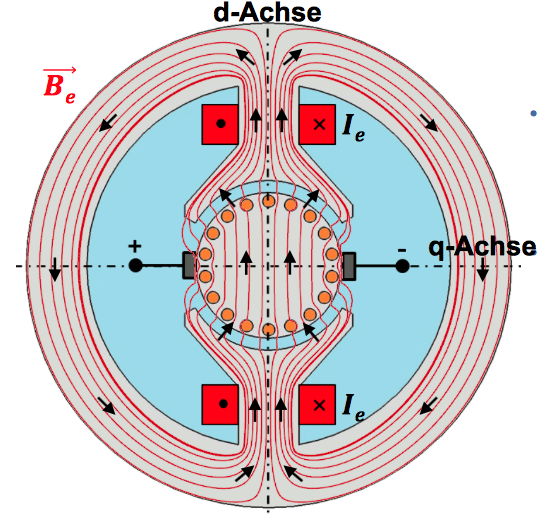
\includegraphics[width = \linewidth]{./Pics/VL45/Ankerruek2}
\end{minipage}

\begin{minipage}{0.4 \linewidth}
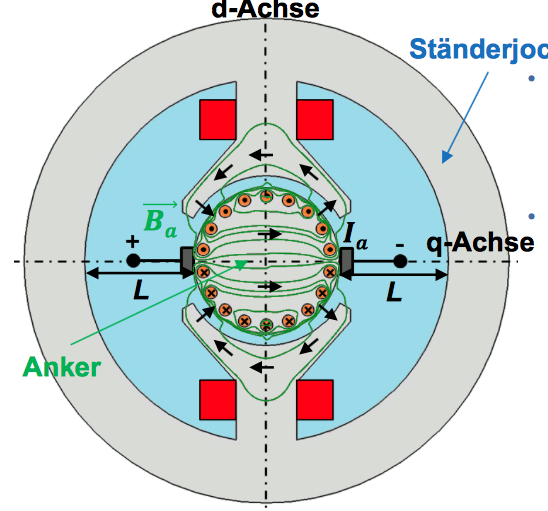
\includegraphics[width = \linewidth]{./Pics/VL45/Ankerruek3}
\end{minipage}
\begin{minipage}{0.6 \linewidth}
\begin{itemize}
\item Der Ankerstrom erzeugt das eigene magnetische Feld, das im Ankerkern parallel zu der q-Achse ausgerichtet ist. 
\item Da in der Richtung der q-Achse der Abstand (L) zwischen dem Anker und dem Ständerjoch sehr gross ist, finden die magnetischen Feldlinien den Rückweg entweder zwischen der Ankerwicklung und der äusseren Ankerfläche (sehr eng) oder durch den Luftspalt und den Polschuh (realtiv breit).
\end{itemize}
\end{minipage}

\begin{minipage}{0.6 \linewidth}
\begin{itemize}
\item Die Wirkung des Ankerfelds ist im Anker und im Luftspalt offenbar am stärksten.
\item Die Verzerrung des magnetischen Gesamtfelds im Anker löst die Verschiebung des Winkels aus, der dem Nulldurchgang der induzierten Ankerspannung entspricht.
\item Wenn der Winkel des Nulldurchgangs der induzierten Nullspannung und die Position der Bürsten nicht übereinander liegen, werden die schlechte Kommutierung und dadurch das Läuferfeuer ausgelöst.
\end{itemize}
\end{minipage}
\begin{minipage}{0.4 \linewidth}
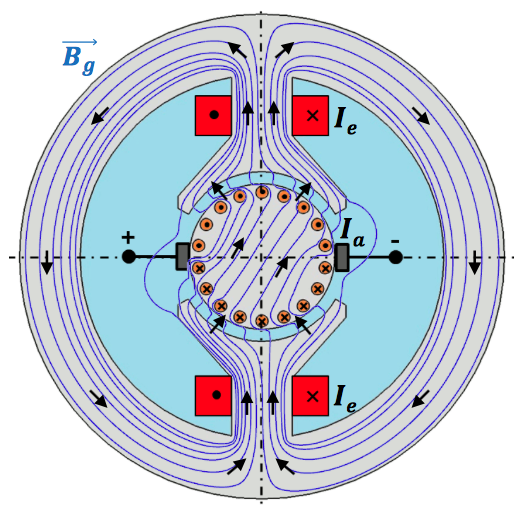
\includegraphics[width = \linewidth]{./Pics/VL45/Ankerruek4}
\end{minipage}

\subsubsection{Kompoundwicklung}
\begin{minipage}{0.4 \linewidth}
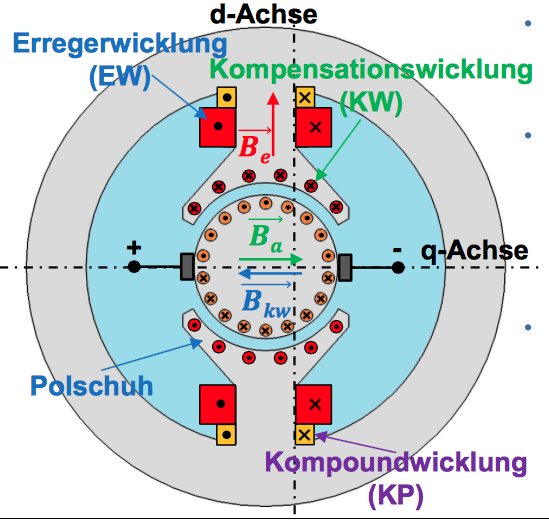
\includegraphics[width = \linewidth]{./Pics/VL45/Kompoundwicklung}
\end{minipage}
\begin{minipage}{0.6 \linewidth}
\begin{itemize}
\item Um die Rückwirkung des Ankerwicklung zu vermindern, wird eine zusätzliche Wicklung, die als Kompensationswicklung (KW)  bekannt ist, im Polshuh des Stators eingesetzt.
\item Der Strom der KW-Wicklung ist so ausgesetzt, dass dessen magnetisches Feld ($B_{kw}$) das Feld der Ankerwicklung aufhebt.
\item Die KW-Wicklung ist konstruktiv sehr aufwändig und damit auch teuer. Deswegen wird sie nur bei Hochleistungsmaschinen verwendet.
\item Die Nuten der KW-Wicklung reduzieren das Hauptfeld $B_e$ (Luft statt Eisen).
\item Um die durch die KW-Wicklung verursachte Hauptfeldschwächung zu kompensieren, wird die Kompoundwicklung (KP) eingesetzt. 
\item Die Hauptfeldkompensation sollte lastabhängig sein. Deswegen fliesst der Ankerstrom auch durch die KP-Wicklung (Reihenschaltung). 
\end{itemize}
\end{minipage}

\subsubsection{Wendepolwicklung}
\begin{minipage}{0.6 \linewidth}
\begin{itemize}
\item Um das Feldverzerrung in der geometrisch neutralen Zone (q-Achse) bei Laständerung zu minimieren und dadurch die Qualität der Kommutierung zu verbessern, wird die Wendepolwicklung (WW) eingesetzt. 
\item Die Wendepolwicklung wird vom Ankerstrom durchflossen, weil die Wirkung der WW-Wicklung lastabhängig sein muss.
\end{itemize}
\end{minipage}
\begin{minipage}{0.4 \linewidth}
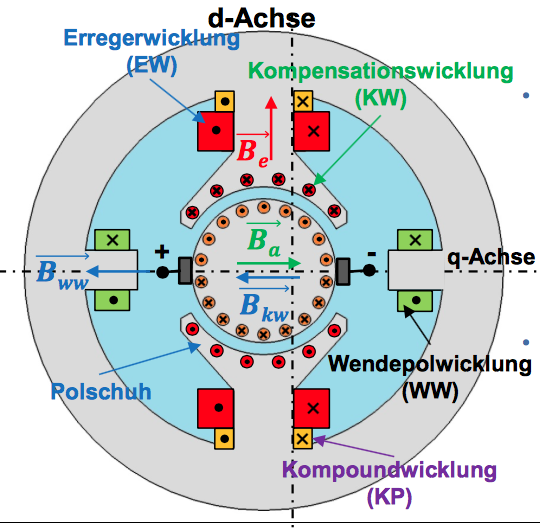
\includegraphics[width = \linewidth]{./Pics/VL45/Wendepolwicklung}
\end{minipage}

\subsection{Arbeitsbereiche und Grenzwerte}

\begin{minipage}{0.4 \linewidth}
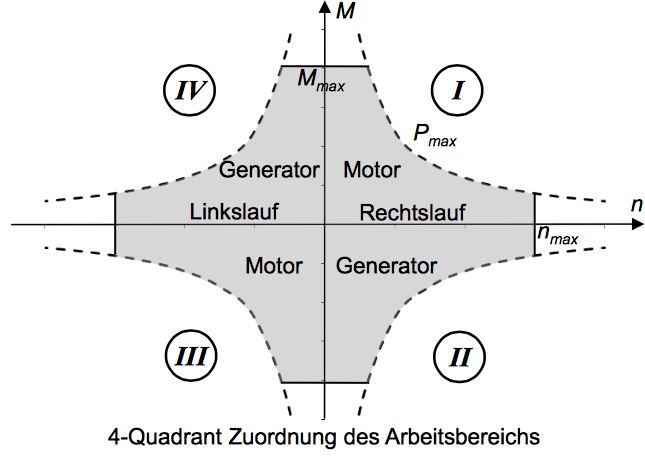
\includegraphics[width = \linewidth]{./Pics/VL45/Arbeitsbereich}
\end{minipage}
\begin{minipage}{0.6 \linewidth}
Im Datenblatt der Maschine werden vom Hersteller die Betriebsgrenzwerte gegeben: \\

$P_{max},M_{max},n_{max},I_{emax}(\Psi_{max}),I_{amax} und U_{amax}$\\

$P = \omega \cdot M = 2 \cdot \pi \cdot n \cdot M$ \\

$M(n) = \frac{P_{max}}{2 \cdot \pi} \cdot \frac{1}{n}$\\
\end{minipage}

\subsection{Nebenschluss und Reihenschluss}
\subsubsection{Nebenschluss}

Die Erreger- und Ankerwicklung werden parallel an die gleiche Spannungsquelle geschaltet. Dei dem Nebenschluss sind die Anker- und Erregerspannung gleich und die Anker- und Erregerstrom unabhängig voneinander.

\begin{minipage}{0.4 \linewidth}
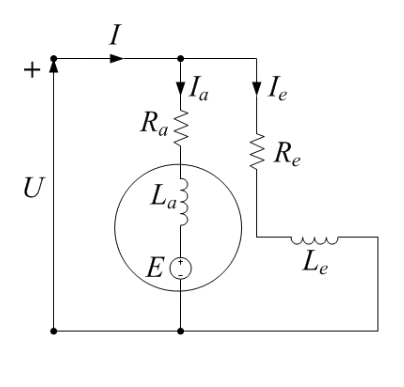
\includegraphics[width = \linewidth]{./Pics/VL45/Nebenschluss}
\end{minipage}
\begin{minipage}{0.6 \linewidth}
Analyse des Drehmoments: \\ 

$M = I_a \cdot \Psi, U = U_a = R_a \cdot I_a + 2 \cdot \pi n \cdot \Psi$ \\

$M = I_a \cdot \Psi = \frac{U \cdot \Psi}{R_a} - \frac{2 \cdot \pi \cdot \Psi^2}{R_a} \cdot n$ \\

Anlaufmoment: \\

$n = 0 \Rightarrow M_a = \frac{U \cdot \Psi}{R_a}$ ($Nm$) \\

Lehrlaufdrehzahl: \\

$M = 0 \Rightarrow n_0 = \frac{U}{2 \cdot \pi \Psi} $ ($\frac{{1}}{s}$)
\end{minipage}

\begin{minipage}{0.4 \linewidth}
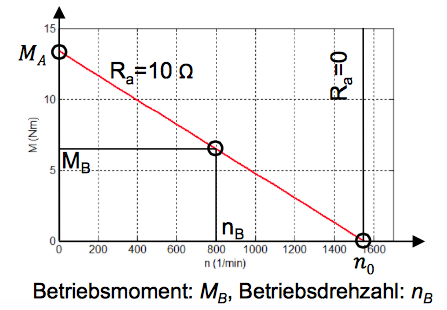
\includegraphics[width = \linewidth]{./Pics/VL45/Nebenschluss2}
\end{minipage}
\begin{minipage}{0.6 \linewidth}
Analyse des Drehmoments: \\

$\frac{M}{M_a} = 1 - \frac{n}{n_0}$\\

$M_a = \frac{U \cdot \Psi}{R_a}$\\

$n_0 = \frac{U}{2 \cdot \pi \cdot \Psi}$
\end{minipage}

\subsubsection{Reihenschluss}
\begin{minipage}{0.3 \linewidth}
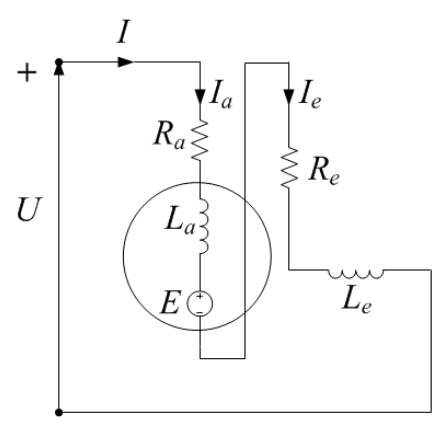
\includegraphics[width = \linewidth]{./Pics/VL45/Reihenschluss}
\end{minipage}
\begin{minipage}{0.7 \linewidth}
Dir Erreger. und Ankerwicklung werden in Serie an die gemeinsame Spannungsquelle geschaltet. Bei dem Reihenschluss sind die Anker- und Erregerstrom gleich und deswegen stark abhängig voneinander. \\

Analyse des Drehmoments: \\

$M = I \cdot \Psi$ \\

$U = (R_a + R_e) \cdot I + 2 \cdot \pi \cdot n \cdot \Psi$ \\

$\Psi = L_e \cdot I$ \\

$M = I \cdot \Psi = L_e (\frac{U}{R_a + R_e + 2 \cdot \pi \cdot n \cdot L_e})^2$ \\

Anlaufmoment: \\

$n = 0 \Rightarrow M_A = \frac{L_e \cdot U^2}{(R_a + R_e)^2}$   $(Nm)$ \\

Bezugsdrehzahl: \\

$n_b = \frac{R_a + R_e}{2 \cdot \pi \cdot L_e}$   $(\frac{1}{s})$
\end{minipage}

\begin{minipage}{0.3 \linewidth}
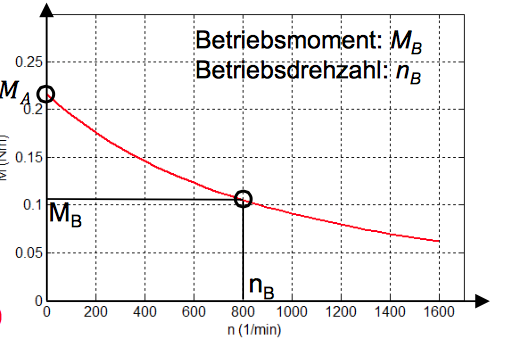
\includegraphics[width = \linewidth]{./Pics/VL45/Reihenschluss2}
\end{minipage}
\begin{minipage}{0.7 \linewidth}
\large{Achtung:} $M \rightarrow 0 \Rightarrow n \rightarrow \inf $\textbf{(Sicherheitsrisiko!)} \\

$\frac{M}{M_A} = \frac{1}{(1 + \frac{n}{n_b})^2} $  \\

$M_A = \frac{L_e \cdot U^2}{(R_a + R_e)^2} $ \\

$n_b = \frac{R_a + R_e}{2 \cdot \pi \cdot L_e}$
\end{minipage}

\subsection{Drehzahlregelung}
\begin{minipage}{0.3 \linewidth}
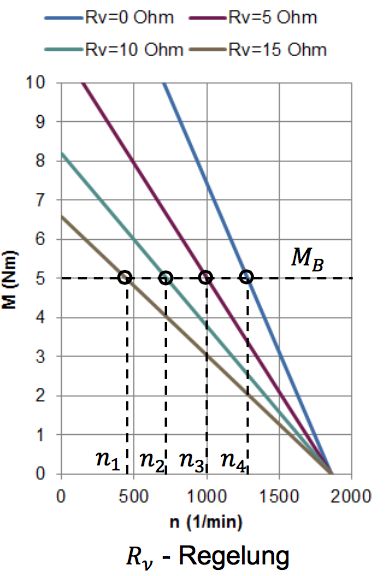
\includegraphics[width = \linewidth]{./Pics/VL45/Drehzahlregelung}
\end{minipage}
\begin{minipage}{0.7 \linewidth}
Die Grundgleichung der Gleichstrommaschine im Nebenschluss: \\

$I_a = \frac{U- 2\cdot\pi \cdot n \cdot \Psi}{R_a}$\\

$M = \frac{U \cdot \Psi}{R_a}- \frac{2\cdot\pi\Psi^2}{R_a}\cdot n$\\

Gemäss den Grundgleichungen sind die Kennlinien $I_a(n)$ und $M(n)$ von $R_a$, $U$ und $\Psi$ stark abhängig. Deswegen wird die Drehzahlregelung durch den zusätzlichen Widerstand $R_v$ im Ankerkreis (verlustreich), durch die Ankerspannung (Verlustarm), oder durch Erregung (Verlustarm) durchgeführt.
\end{minipage}

\begin{minipage}{0.3 \linewidth}
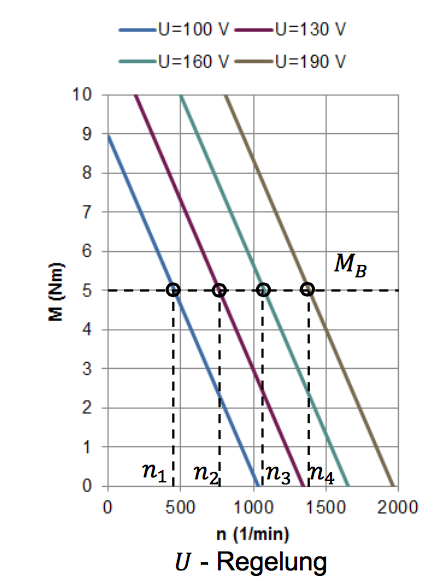
\includegraphics[width = \linewidth]{./Pics/VL45/Drehzahlregelung2}
\end{minipage}
\begin{minipage}{0.3 \linewidth}
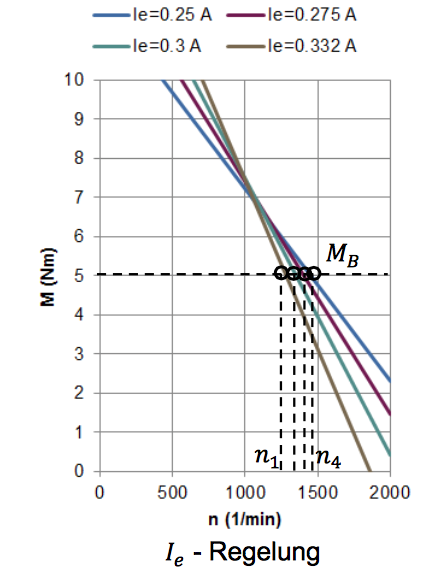
\includegraphics[width = \linewidth]{./Pics/VL45/Drehzahlregelung3}
\end{minipage}

\subsection{Anlauf}
Wegen der Stabilität des Netzwerks muss der Anlaufstrom der Gleichstrommotoren mit einer Leistung über 2 kW begrenzt werden. Ein beispiel der Anlaufstrombegrenzung durch die $R_v$-Regelung sieht so aus: \\

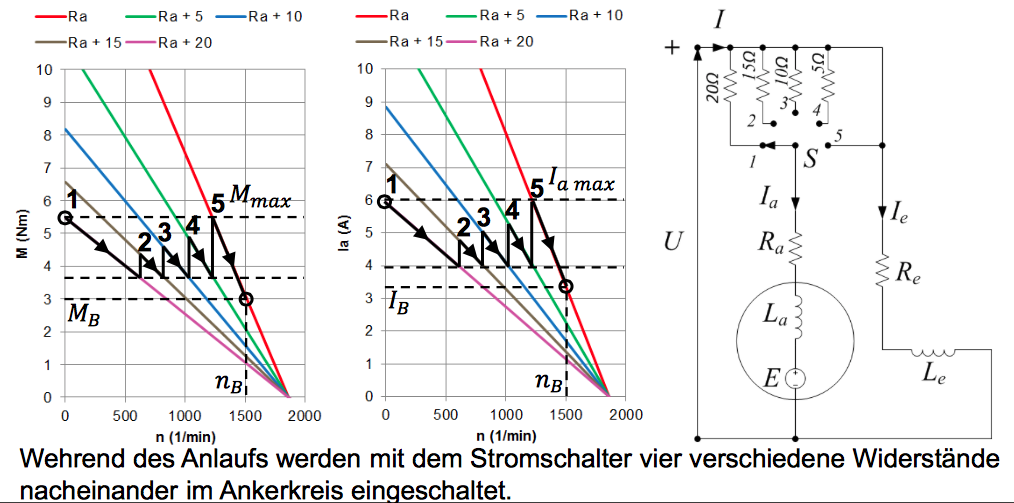
\includegraphics[width = 0.8 \linewidth]{./Pics/VL45/Anlauf}

\subsection{Anwendungsbereiche und Schlussanmerkungen}
\begin{itemize}
\item Die Gleichstrommaschine sind konstruktiv sehr kompliziert und damit auch sehr teuer.
\item Die Gleichstrommaschine mit Fremd-, Neben- und Permanenterregung werden heute nur als Motoren eingesetzt.
\item Die Anwendung in den lokalen Gleichstromnetzen: Fahrzeuge, Schiffe, Batterie-gespeiste Geräte, usw.
\item Spezielle Anwendung wobei stetige Drehzahlregelung erforderlich ist:
\begin{compactitem}
\item Werkzeugmaschine
\item Haspeln
\item Drehrohröfen
\item Papiermaschinen
\item Textilmaschinen,
\item usw.
\end{compactitem}
\item Nebenschluss-GSM: 0.25-3000 kW, 0-3000 $min^{-1}$ (für regelbare Antriebe)
\item Reihenschluss-GSM: 0.5 -1000 kW, 0-10'000 $min^{-1}$ (für Fahrzeugantriebe)
\end{itemize}